\newcommand{\ContrLearnMrrAndMapResultsTable}{
	\begin{table}[H]
		\centering
		\begin{tabular}{|P{2cm}||P{3,2cm} P{3,2cm} P{3,2cm}|}
			\hline
			& Joint Embedding Contrastive Model & Proposed Model Contrastive Model & Contrastive Model Only \\
			\hline
			MRR & 0.506$\pm$0.008 & \textBF{0.509$\pm$0.002} & 0.503$\pm$0.011 \\
			MAP & 0.441$\pm$0.003 & \textBF{0.443$\pm$0.002} & 0.437$\pm$0.004 \\
			\hline
		\end{tabular}
		\caption[Contrastive Model family ranking MRR and MAP scores]{Mean and standard deviation MRR (Mean Reciprocal Rank) and MAP (Mean Average Precision) results obtained by evaluating the Contrastive Model based on the \textbf{Joint Embedding} and \textbf{Proposed Model} along with a Contrastive Model with no \textit{Transfer Learning} applied (\textit{Contrastive Model Only}) on the Family Ranking task. Results were aggregated over \textBF{3} training runs with different weight initializations and minibatch orderings. Best results are shown in \textbf{bold}.} \label{tab:ContrLearnMrrAndMapResults}
	\end{table}
}

\newcommand{\ContrLearnAccuracyResultsTable}{
	\begin{table}[H]
		\centering
		\begin{tabular}{|P{2cm}||P{3,2cm} P{3,2cm} P{3,2cm}|}
			\hline
			& Joint Embedding Contrastive Model (with $k=9$) & Proposed Model Contrastive Model (with $k=5$) & Contrastive Model only (with $k=11$) \\
			\hline
			Accuracy & 0.427$\pm$0.003 & \textBF{0.431$\pm$0.007} & 0.415$\pm$0.013 \\
			\hline
		\end{tabular}
		\caption[Contrastive Model Accuracy Results]{Mean and Standard deviation of the accuracy obtained by evaluating the Contrastive Model based on the \textbf{Joint Embedding} and \textbf{Proposed Model} along with a Contrastive Model with no \textit{Transfer Learning} applied (\textit{Contrastive Model Only}) on the family classification task. Results were aggregated over \textBF{3} training runs with different weight initializations and minibatch orderings. Best results are shown in \textbf{bold}.} \label{tab:ContrLearnAccuracyResults}
	\end{table}
}

\newcommand{\ContrLearnScoresTable}{
	\begin{table}[H]
		\centering
		\begin{tabular}{|P{1,8cm}|P{1,3cm}||P{3cm} P{3cm} P{3cm}|}
			\hline
			& & Joint Embedding Contrastive Model (with $k=9$) & Proposed Model Contrastive Model (with $k=5$) & Contrastive Model only (with $k=11$) \\
			\hline
			\multirow{3}{4em}{Jaccard Similarity} & Micro & 0.271$\pm$0.002 & \textBF{0.274$\pm$0,006} & 0.262$\pm$0.010 \\
			& Macro & 0.310$\pm$0.006 & \textBF{0.313$\pm$0.003} & 0.292$\pm$0.008 \\
			& Weighted & 0.310$\pm$0.007 & \textBF{0.314$\pm$0.003} & 0.291$\pm$0.009 \\
			\hline
			\multirow{3}{4em}{Recall} & Micro & 0.427$\pm$0.003 & \textBF{0.431$\pm$0.007} & 0.415$\pm$0.013 \\
			& Macro & 0.427$\pm$0.002 & \textBF{0.430$\pm$0.007} & 0.415$\pm$0.012 \\
			& Weighted & 0.427$\pm$0.003 & \textBF{0.431$\pm$0.007} & 0.415$\pm$0.013 \\
			\hline
			\multirow{3}{4em}{Precision} & Micro & 0.427$\pm$0.003 & \textBF{0.431$\pm$0.007} & 0.415$\pm$0.013 \\
			& Macro & 0.481$\pm$0.003 & \textBF{0.502$\pm$0.008} & 0.469$\pm$0.014 \\
			& Weighted & 0.481$\pm$0.004 & \textBF{0.501$\pm$0.009} & 0.469$\pm$0.014 \\
			\hline
			\multirow{3}{4em}{F1-score} & Micro & 0.427$\pm$0.003 & \textBF{0.431$\pm$0.007} & 0.415$\pm$0.013 \\
			& Macro & 0.433$\pm$0.006 & \textBF{0.434$\pm$0.001} & 0.400$\pm$0.003 \\
			& Weighted & 0.433$\pm$0.007 & \textBF{0.435$\pm$0.001} & 0.400$\pm$0.004 \\
			\hline
		\end{tabular}
		\caption[Contrastive Model Scores]{Mean and Standard deviation of the multi-class classification scores obtained by evaluating the 2 Contrastive Models obtained by transferring the knowledge from a previous training run on the Sorel-20m dataset of the \textbf{Joint Embedding} and \textbf{Proposed Model} implementations, respectively, along with a Contrastive Model with no \textit{Transfer Learning} applied (\textit{Contrastive Model Only}) on the family classification task using the k-NN algorithm. Results were aggregated over \textBF{3} training runs with different weight initializations and minibatch orderings. Best results are shown in \textbf{bold}.} \label{tab:ContrLearnScoresTable}
	\end{table}
}

\newcommand{\ContrLearnJointEmbeddingConfusionMatrix}{
	\begin{figure}[H]
		\vspace*{-0.5cm}
		\centering
		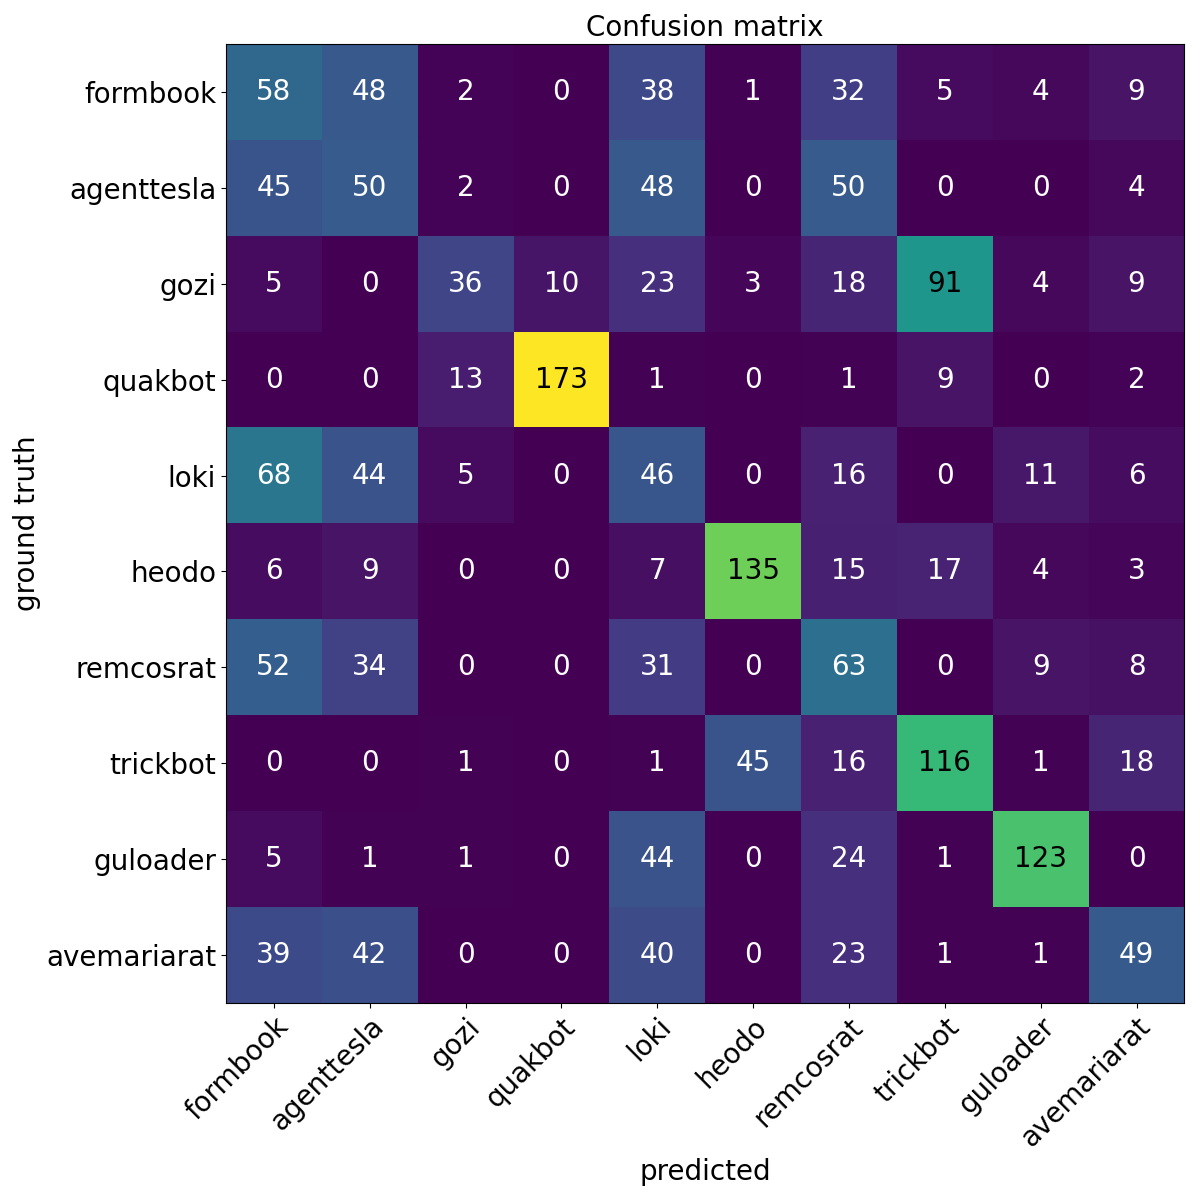
\includegraphics[width=0.7\textwidth]{./results/joint_embedding_contr_learn_9-nn_confusion_matrix.png}
		\vspace*{-0.2cm}
		\caption[Contrastive Model based on Joint Embedding Confusion Matrix]{Confusion Matrix resulting from the evaluation of the Contrastive Model obtained by transferring the knowledge from a previous \textbf{Joint Embedding} model training run on the Sorel-20m dataset on the family classification task using the k-NN algorithm with $k=9$.}
		\label{fig:ContrLearnJointEmbeddingConfusionMatrix}
	\end{figure}
}

\newcommand{\ContrLearnProposedModelConfusionMatrix}{
	\begin{figure}[H]
		\vspace*{-0.5cm}
		\centering
		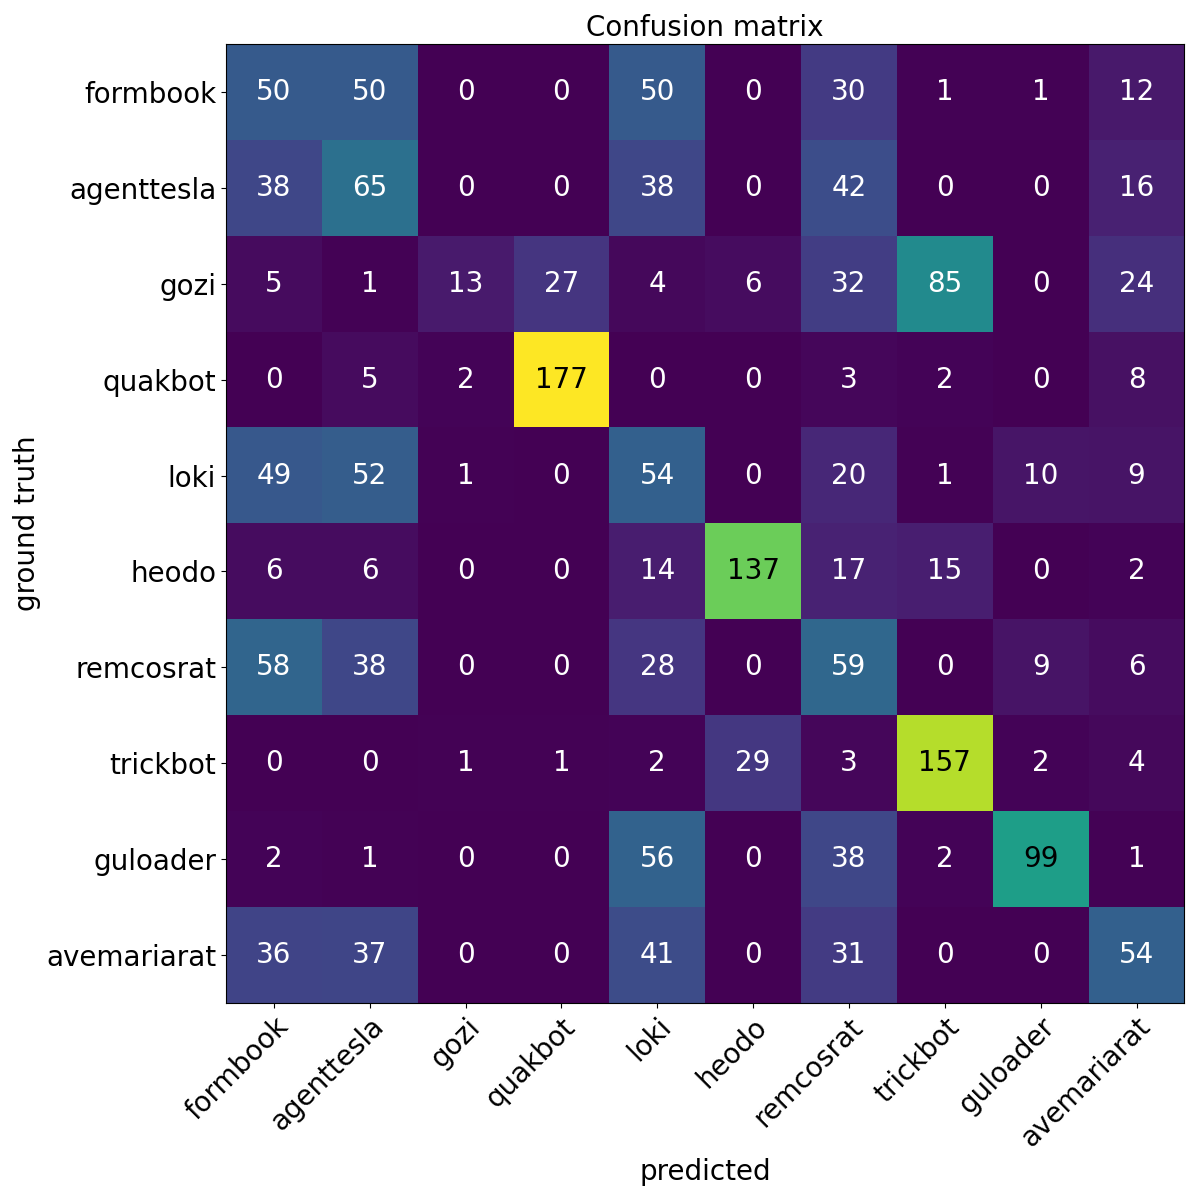
\includegraphics[width=0.7\textwidth]{./results/proposed_model_contr_learn_5-nn_confusion_matrix.png}
		\vspace*{-0.2cm}
		\caption[Contrastive Model based on Proposed Model Confusion Matrix]{Confusion Matrix resulting from the evaluation of the Contrastive Model obtained by transferring the knowledge from a previous \textbf{Proposed Model} training run on the Sorel-20m dataset on the family classification task using the k-NN algorithm with $k=5$.}
		\label{fig:ContrLearnProposedModelConfusionMatrix}
	\end{figure}
}

\newcommand{\ContrLearnOnlyConfusionMatrix}{
	\begin{figure}[H]
		\vspace*{-0.5cm}
		\centering
		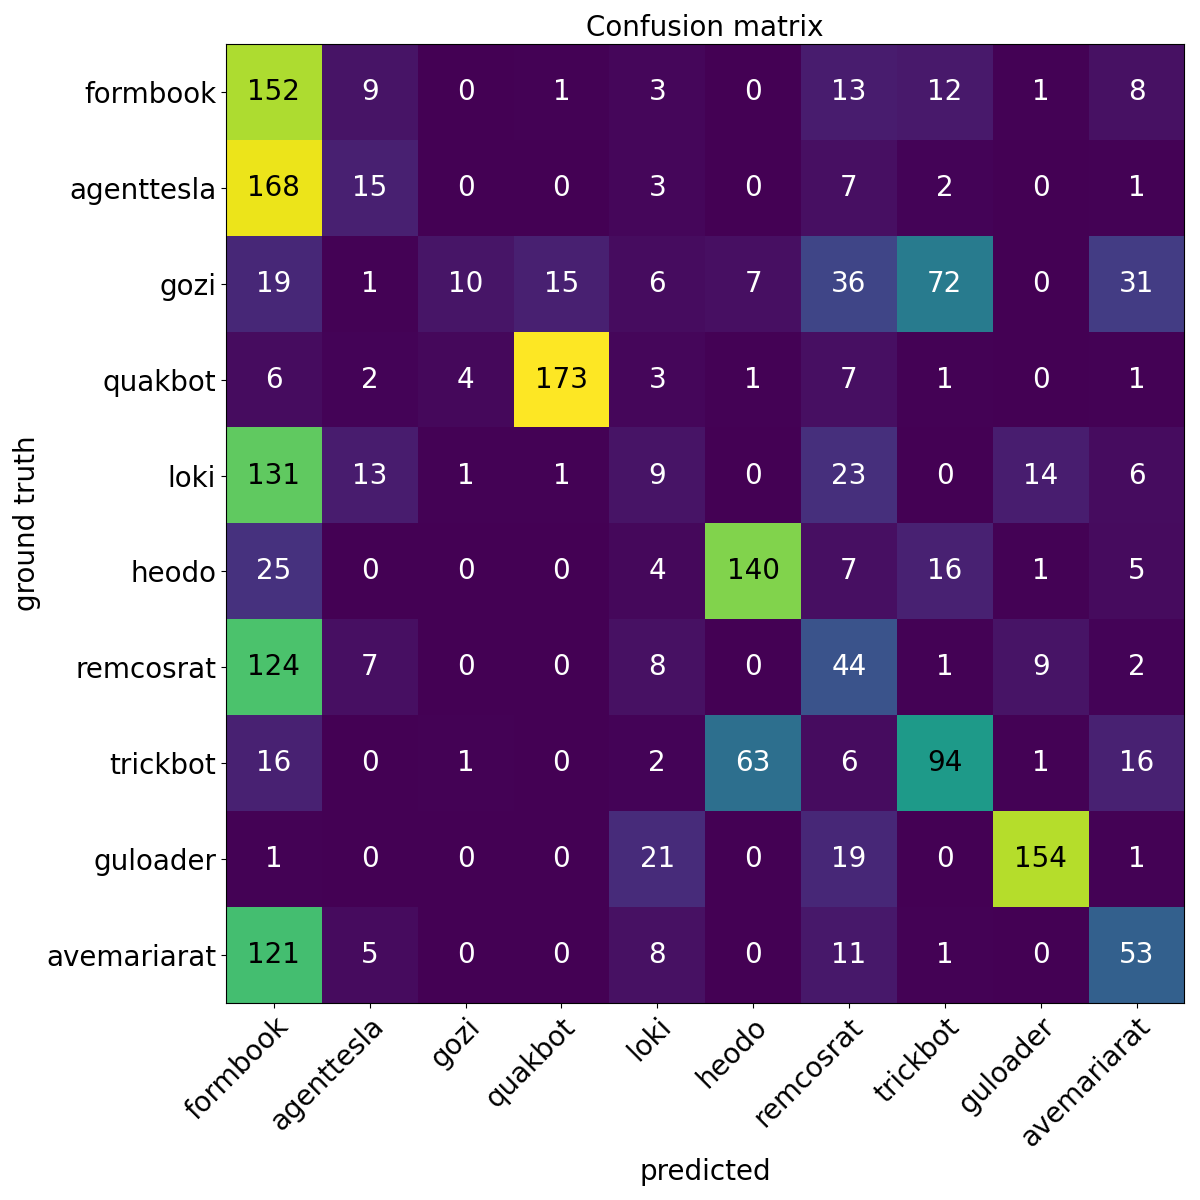
\includegraphics[width=0.7\textwidth]{./results/contrastive_model_only_contr_learn_11-nn_confusion_matrix.png}
		\vspace*{-0.2cm}
		\caption[Contrastive Model Only Joint Embedding Confusion Matrix]{Confusion Matrix resulting from the evaluation of the Contrastive Model trained from scratch (with no transfer learning) on the family classification task using the k-NN algorithm with $k=11$.}
		\label{fig:ContrLearnOnlyConfusionMatrix}
	\end{figure}
}

\newcommand{\ContrLearnMaxApExampleRankTable}{
	\begin{table}[H]
		\centering
		\begin{tabular}{|P{1,8cm}||P{1,7cm} P{1,2cm} P{2cm}|P{1,7cm} P{1,2cm} P{2cm}|}
			\hline
			Max AP & \multicolumn{3}{c|}{ALOHA (M/B)} & \multicolumn{3}{c|}{ALOHA} \\
			& Sha256 & Label & Family & Sha256 & Label & Family \\
			\hline
			Query & 24133d.. & 0 & formbook & e3639a.. & 0 & formbook \\
			\hline
			0 & 8fea1e.. & 3 & quakbot & \textBF{6f16d3}.. & \textBF{0} & \textBF{formbook} \\
			1 & \textBF{02ad1e}.. & \textBF{0} & \textBF{formbook} & \textBF{0655ee}.. & \textBF{0} & \textBF{formbook} \\
			2 & \textBF{8da806}.. & \textBF{0} & \textBF{formbook} & \textBF{40f8cf}.. & \textBF{0} & \textBF{formbook} \\
			3 & 0c95f0.. & 8 & guloader & \textBF{f7c1ec}.. & \textBF{0} & \textBF{formbook} \\
			4 & 95fa71.. & 9 & avemariarat & 620c36.. & 2 & gozi \\
			5 & 4b8466.. & 6 & remcosrat & 38e003.. & 6 & remcosrat \\
			6 & \textBF{191008}.. & \textBF{0} & \textBF{formbook} & \textBF{93e548}.. & \textBF{0} & \textBF{formbook} \\
			7 & 768da5.. & 9 & avemariarat & 1ddaae.. & 4 & loki \\
			8 & \textBF{e92575}.. & \textBF{0} & \textBF{formbook} & 5b9f32.. & 3 & quakbot \\
			9 & f0cae3.. & 3 & quakbot & 83d036.. & 4 & loki \\
			\hline
			Max AP & \multicolumn{3}{c|}{0.186} & \multicolumn{3}{c|}{0.174} \\
			\hline
			Next & \multicolumn{3}{c|}{position 14} & \multicolumn{3}{c|}{position 10} \\
			\hline
			\hline
			Max AP & \multicolumn{3}{c|}{Joint Embedding} & \multicolumn{3}{c|}{Proposed Model} \\
			& Sha256 & Label & Family & Sha256 & Label & Family \\
			\hline
			Query & c0a92a.. & 6 & remcosrat & 389ec4.. & 7 & trickbot \\
			\hline
			0 & \textBF{21f9ef}.. & \textBF{6} & \textBF{remcosrat} & \textBF{aa447e}.. & \textBF{7} & \textBF{trickbot} \\
			1 & \textBF{49c7a5}.. & \textBF{6} & \textBF{remcosrat} & \textBF{cbe743}.. & \textBF{7} & \textBF{trickbot} \\
			2 & f75cb4.. & 2 & gozi & 8dc3da.. & 6 & remcosrat \\
			3 & \textBF{91b004}.. & \textBF{6} & \textBF{remcosrat} & \textBF{e37438}.. & \textBF{7} & \textBF{trickbot} \\
			4 & 2d54d3.. & 3 & quakbot & \textBF{2cadf2}.. & \textBF{7} & \textBF{trickbot} \\
			5 & f86765.. & 9 & avemariarat & 545bc3.. & 8 & guloader \\
			6 & 0ea373.. & 0 & formbook & \textBF{b56a1e}.. & \textBF{7} & \textBF{trickbot} \\
			7 & \textBF{4a9558}.. & \textBF{6} & \textBF{remcosrat} & e14108.. & 6 & remcosrat \\
			8 & 019f79.. & 7 & trickbot & 80e880.. & 2 & gozi \\
			9 & a2f8c1.. & 9 & avemariarat & \textBF{4688b8}.. & \textBF{7} & \textBF{trickbot} \\
			\hline
			Max AP & \multicolumn{3}{c|}{0.190} & \multicolumn{3}{c|}{0.183} \\
			\hline
			Next & \multicolumn{3}{c|}{position 11} & \multicolumn{3}{c|}{position 17} \\
			\hline
		\end{tabular}
		\caption[Family ranking max AP example]{\textBF{ALOHA (M/B) Embedding}, \textBF{ALOHA}, \textBF{Joint Embedding} and \textBF{Proposed Model} example rankings (limited to the first 10 samples) having the maximum Average Precision (max AP). The elements matching the query sample are shown in \textbf{bold}. The last line of each table indicates the position in the ranking where to find the next element belonging to the same family as the query sample.} \label{tab:ContrLearnMaxApExampleRank}
	\end{table}
}